\section{Input data definition}
\subsection{Exposure model definition}
All risk calculators in OpenQuake require an exposure model that needs to be stored in NRML. Common to all of the assets stored in a given exposure model, the following metadata needs to be provided, as described below: 

\begin{itemize}
\item  \Verb+id+: a unique key used to identify the exposure model within OpenQuake;
\item  \Verb+assetCategory+: a string used to define the type of assets being stored (e.g: buildings, population);
\item  \Verb+areaType+: flag defining the way this parameter is being provided, as explained later in this section; 
\item  \Verb+areaUnits+: attribute defining the units used to measure the area; 
\item  \Verb+stcoType+: flag defining the way the structural cost is being provided, as explained later in this section; 
\item  \Verb+stcoUnits+: attribute defining the units used to measure the structural cost;
\item  \Verb+recoType+: flag defining the way the retrofitting cost is being provided, as explained later in this section; 
\item  \Verb+recoUnits+: attribute defining the units used to measure the retrofitting cost;
\item  \Verb+description+: brief string with further information about the exposure model;
\item  \Verb+taxonomySource+: attribute used to define the taxonomy system being used to classify the assets;
\end{itemize}

The way the information about the characteristics of the assets in an exposure model are  stored can vary strongly depending on the authority in charge of compiling the data. As an example, if national census information is used to estimated the distribution of assets in a given region, it is likely that the number of buildings per unit of area will be used to define the dataset. In the other hand, if simplified methodologies based on population distribution are used for this purpose, then it is likely that the built up area or economic value of each building typology will be used. Thus, the following set of attributes were included in the latest version of the schema for the exposure model:

\begin{itemize}
\item  \Verb+number+: number of assets for a given location;
\item  \Verb+area+: area of the asset typology;
\item  \Verb+stco+: structural cost of the asset (i.e. replacement cost); 
\item  \Verb+reco+: retrofitting cost of the asset. 
\end{itemize}

While the attribute \Verb+number+ might be a rather simple parameter, the other two can be considerably ambiguous as different ways to define them might be used. With regards to the attribute \Verb+area+, one can either choose to provide the aggregated built up area of a certain building typology per location or the average built up area for a single unit. Similarly, the \Verb+stco+ can also be defined as the aggregated economic value (replacement cost for all the asset at the given location), the cost of replacing a single unit or even the replacement cost for unit of area. For the purposes of performing a benefit/cost analysis, it is also necessary to define the retrofitting cost (\Verb+reco+). This parameter is being handled in the same manner as the structural cost. Thus, it can be defined as the aggregated retrofitting cost, the average cost per unit of area, or as the average cost for a single unit. 

To establish the way these three attributes are being defined within the exposure model, three flags have been introduced in the schema model:  \Verb+areaType+, \Verb+stcoType+ and \Verb+recoType+.

Notice that since the attribute \Verb+number+ always represents the same quantity (number of assets in a given location), no flag providing further information about this attribute was introduced. Further information regarding the parameters that are currently being used to define the exposure elements can be found in the OpenQuake book. In order to clarify this methodology, several examples are presented later in this section.

Finally, a pair of coordinates (longitude and latitude) needs to be provided to define the location of each asset.The way this information is being stored is constantly being modified, as further feedback from users and experts is received. Hence, it is important to understand which version of NRML OpenQuake is using, in order to avoid incompatibility issues. NRML is already in its third version (0.4) and documentation about each release can be found on Github. Several examples of exposure models containing different types of information are presented now. Users will notice that some of the attributes are marked with a "\Verb+gml+" tag, which means that these parameters must follow the Geography Markup Language grammar, developed by the Open Geospatial Consortium.\

\paragraph{Example 1}
This example is comprised by an exposure model in which the aggregated economic value of each building typology for a set of locations is directly provided.

\begin{Verbatim}[frame=single, commandchars=\\\{\}, samepage=false]
<?xml version="1.0" encoding="UTF-8"?>
<nrml xmlns:gml="http://www.opengis.net/gml"
      xmlns="http://openquake.org/xmlns/nrml/0.4">
<\textcolor{red}{exposureModel} gml:id="ep">
    <\textcolor{green}{exposureList} gml:id="Nepal_13_1" assetCategory="buildings" 
    stcoUnit="EUR" stcoType="aggregated" recoUnit="EUR" 
    recoType="aggregated">
    <gml:description>Buildings in Nepal</gml:description>
    <taxonomySource>Nepal taxonomy</taxonomySource>
        <\textcolor{blue}{assetDefinition} gml:id="asset1">
            <site>
               <gml:Point srsName="epsg:4326">
               <gml:pos>15.22 38.80</gml:pos>
               </gml:Point>
            </site>
            <taxonomy>URM</taxonomy>
            <stco> 500.0 </stco>
            <reco> 50.0 </reco>
        <\textcolor{blue}{/assetDefinition} 
        ...
        <\textcolor{blue}{assetDefinition} gml:id="asset999">
            <site>
               <gml:Point srsName="epsg:4326">
	      <gml:pos>15.23 38.95</gml:pos>
	      </gml:Point>
	   </site>
	   <taxonomy>RC</taxonomy>
	   <stco> 700.0 </stco>
	   <reco> 70.0 </reco>
        <\textcolor{blue}{/assetDefinition}> 
    <\textcolor{green}{/exposureList}>
<\textcolor{red}{/exposureModel}>
</nrml>
\end{Verbatim}

Each asset is uniquely identified by its \Verb+id+, which is used by OpenQuake to relate each asset with the associated results (e.g.: loss curves). Then, a pair of coordinates (latitude and longitude) for a \Verb+site+ is defined. This position (\Verb+pos+) and the associated geographical projection (\Verb+srsName+) need to be provided in the \Verb+Point+ attribute. Each asset must to be classified according to a \Verb+taxonomy+, so that OpenQuake is capable of employing the appropriate vulnerability or fragility function in the risk calculations. Finally, the value of the asset is stored in the \Verb+stco+ attribute. In this case, the aggregated economic value for the assets at each location if provided directly, so there is no need of defining other attributes such as \Verb+number+ or \Verb+area+. This mode of representing an exposure model is probably simplest way.\\ 

\paragraph{Example 2}
This example is comprised by an exposure model containing the number of buildings at each location, and the associated replacement and retrofitting cost per unit of each building typology.

\begin{Verbatim}[frame=single, commandchars=\\\{\}, samepage=false]
<?xml version="1.0" encoding="UTF-8"?>
<nrml xmlns:gml="http://www.opengis.net/gml"
      xmlns="http://openquake.org/xmlns/nrml/0.4">
<\textcolor{red}{exposureModel} gml:id="ep">
    <\textcolor{green}{exposureList} gml:id="Nepal_13_2" assetCategory="buildings" 
    stcoUnit="EUR" stcoType="per_asset" recoUnit="EUR" 
    recoType="per_asset">
    <gml:description>Buildings in Nepal</gml:description>
    <taxonomySource>Nepal taxonomy</taxonomySource>
        <\textcolor{blue}{assetDefinition} gml:id="asset1">
            <site>
               <gml:Point srsName="epsg:4326">
               <gml:pos>15.22 38.80</gml:pos>
               </gml:Point>
            </site>
            <taxonomy>URM</taxonomy>
            <number> 10 </number>
            <stco> 50.0 </stco>
            <reco> 5.0 </reco>
        <\textcolor{blue}{/assetDefinition} 
        ...
        <\textcolor{blue}{assetDefinition} gml:id="asset999">
            <site>
               <gml:Point srsName="epsg:4326">
	      <gml:pos>15.23 38.95</gml:pos>
	      </gml:Point>
	   </site>
	   <taxonomy>RC</taxonomy>
            <number> 5 </number>
	   <stco> 140.0 </stco>
	   <reco> 14.0 </reco>
        <\textcolor{blue}{/assetDefinition}> 
    <\textcolor{green}{/exposureList}>
<\textcolor{red}{/exposureModel}>
</nrml>
\end{Verbatim}

In this example, the economic and retrofitting value of each asset is not provided directly, as happened in the previous example. In order to carry out the risk calculations in which the economic and retrofitting value of each asset is required, OpenQuake multiplies for each asset, the number of buildings by its replacement cost. Notice that in this case, there is no need of specifying the attribute \Verb+area+. 

\paragraph{Example 3}
This example is comprised by an exposure model containing the built up area of each building typology for a set of locations, and the associated replacement cost per area.

\begin{Verbatim}[frame=single, commandchars=\\\{\}, samepage=false]
<?xml version="1.0" encoding="UTF-8"?>
<nrml xmlns:gml="http://www.opengis.net/gml"
      xmlns="http://openquake.org/xmlns/nrml/0.4">
<\textcolor{red}{exposureModel} gml:id="ep">
    <\textcolor{green}{exposureList} gml:id="Nepal_13_3" assetCategory="buildings" 
    stcoUnit="EUR/m2" stcoType="per_area" recoUnit="EUR/m2" 
    recoType="per_area" areaUnit="m2" areaType="aggregated">
    <gml:description>Buildings in Nepal</gml:description>
    <taxonomySource>Nepal taxonomy</taxonomySource>
        <\textcolor{blue}{assetDefinition} gml:id="asset1">
            <site>
               <gml:Point srsName="epsg:4326">
               <gml:pos>15.22 38.80</gml:pos>
               </gml:Point>
            </site>
            <taxonomy>URM</taxonomy>
            <area> 10000 </area>
            <stco> 400.0 </stco>
            <reco> 40.0 </reco>
        <\textcolor{blue}{/assetDefinition} 
        ...
        <\textcolor{blue}{assetDefinition} gml:id="asset999">
            <site>
               <gml:Point srsName="epsg:4326">
	      <gml:pos>15.23 38.95</gml:pos>
	      </gml:Point>
	   </site>
	   <taxonomy>RC</taxonomy>
            <area> 20000 </area>
            <stco> 500.0 </stco>
            <reco> 50.0 </reco>
        <\textcolor{blue}{/assetDefinition}> 
    <\textcolor{green}{/exposureList}>
<\textcolor{red}{/exposureModel}>
</nrml>
\end{Verbatim}

Once again, OpenQuake needs to carry out some calculations in order to compute the economic value per asset. In this case, this value is computed by multiplying the aggregated built up area for each building typology, by the associated replacement or retrofitting cost per unit of area. Notice that in this case, there is no need of specifying the attribute \Verb+number+.

 \paragraph{Example 4}
This example is comprised by an exposure model containing the number of buildings for each location, the average built up area per unit and the associated replacement cost per area. 

\begin{Verbatim}[frame=single, commandchars=\\\{\}, samepage=false]
<?xml version="1.0" encoding="UTF-8"?>
<nrml xmlns:gml="http://www.opengis.net/gml"
      xmlns="http://openquake.org/xmlns/nrml/0.4">
<\textcolor{red}{exposureModel} gml:id="ep">
    <\textcolor{green}{exposureList} gml:id="Nepal13_04" assetCategory="buildings" 
    stcoUnit="EUR/m2" stcoType="per_area" recoUnit="EUR/m2" 
    recoType="per_area" areaUnit="m2" areaType="per_asset">
    <gml:description>Buildings in Nepal</gml:description>
    <taxonomySource>Nepal taxonomy</taxonomySource>
        <\textcolor{blue}{assetDefinition} gml:id="asset1">
            <site>
               <gml:Point srsName="epsg:4326">
               <gml:pos>15.22 38.80</gml:pos>
               </gml:Point>
            </site>
            <taxonomy>URM</taxonomy>
            <number> 10 </number>
            <area> 100.0 </area>
            <stco> 400.0 </stco>
            <reco> 40.0 </reco>
        <\textcolor{blue}{/assetDefinition} 
        ...
        <\textcolor{blue}{assetDefinition} gml:id="asset999">
            <site>
               <gml:Point srsName="epsg:4326">
	      <gml:pos>15.23 38.95</gml:pos>
	      </gml:Point>
	   </site>
	   <taxonomy>RC</taxonomy>
            <number> 5 </number>
            <area> 150.0 </area>
            <stco> 500.0 </stco>
            <reco> 50.0 </reco>
        <\textcolor{blue}{/assetDefinition}> 
    <\textcolor{green}{/exposureList}>
<\textcolor{red}{/exposureModel}>
</nrml>
\end{Verbatim}

In this example, OpenQuake will make use of all the parameters to estimate the economic and retrofitting value for each asset, by multiplying the number of buildings by its average built up area, and then by the respective replacement or retrofitting cost per unit of area. 

\paragraph{Example 5}
This example is comprised by an exposure model containing population distribution.

\begin{Verbatim}[frame=single, commandchars=\\\{\}, samepage=false]
<?xml version="1.0" encoding="UTF-8"?>
<nrml xmlns:gml="http://www.opengis.net/gml"
      xmlns="http://openquake.org/xmlns/nrml/0.4">
<\textcolor{red}{exposureModel} gml:id="ep">
    <\textcolor{green}{exposureList} gml:id="Nepal13_5" assetCategory="population">
    <gml:description>Population in Nepal</gml:description>
    <taxonomySource>Nepal taxonomy</taxonomySource>
        <\textcolor{blue}{assetDefinition} gml:id="asset1">
            <site>
               <gml:Point srsName="epsg:4326">
               <gml:pos>15.22 38.80</gml:pos>
               </gml:Point>
            </site>
            <taxonomy>VF1</taxonomy>
            <number> 200 </number>
        <\textcolor{blue}{/assetDefinition} 
        ...
        <\textcolor{blue}{assetDefinition} gml:id="asset999">
            <site>
               <gml:Point srsName="epsg:4326">
	      <gml:pos>15.23 38.95</gml:pos>
	      </gml:Point>
	   </site>
	   <taxonomy>VF2</taxonomy>
            <number> 100 </number>
        <\textcolor{blue}{/assetDefinition}> 
    <\textcolor{green}{/exposureList}>
<\textcolor{red}{/exposureModel}>
</nrml>
\end{Verbatim}

In this final example, OpenQuake will required population distribution instead of building economic value, hence, only the attribute \Verb+number+ needs to be provided. Notice that in order for OpenQuake recognize that human losses are going to be estimated rather than economic losses, the attribute  \Verb+assetCategory+ needs to be set to  \Verb+population+.  
 
As a part of the Modeller's toolkit development, scripts capable of converting information about the assets stored in Excel or ASCII files into NRML have been developed. 

\subsection{Physical vulnerability model definition}
In this section, the NRML schema for the vulnerability model is described in detail. In order to do so, a graphical representation of a vulnerability model (mean loss ratio for a set of intensity measure levels) is illustrated in Figure \ref{fig:vulModel}, and the equivalent NRML file is then presented. Note that although the uncertainty for each loss ratio is not represented in the aforementioned figure, it has been considered in the input NRLM file, by means of a coefficient of variation per loss ratio. This model is composed by two discrete vulnerability functions and uses spectral acceleration for a certain period. 

\begin{figure}[ht]
\centering
\includegraphics[width=10cm,height=6cm]{./figures/risk/vulnerabilityModel.eps}
\caption{Graphical representation of a vulnerability model.}
\label{fig:vulModel}
\end{figure}

Each component of the associated NRML file is presented herein:
 
\begin{Verbatim}[frame=single, commandchars=\\\{\}, samepage=true]
<?xml version="1.0" encoding="UTF-8"?>
<nrml xmlns:gml="http://www.opengis.net/gml"
      xmlns="http://openquake.org/xmlns/nrml/0.4">
<\textcolor{red}{vulnerabilityModel}>
    <\textcolor{green}{discreteVulnerabilitySet} vulnerabilitySetID="OpenQuake2013"	
    assetCategory="buildings"    lossCategory="economic loss">
        ...
\end{Verbatim}

At the top of the NRML schema, the following metadata are being stored:
\begin{itemize}
\item  \Verb+vulnerabilitySetID+: A unique key used to identify the vulnerability model instance within OpenQuake;
\item  \Verb+assetCategory+: An attribute that describes the asset typology (e.g.: population, buildings, contents);
\item  \Verb+lossCategory+: An attribute that describes the type of loss suffered by the assetCategory (e.g.: fatalities, collapse, economic loss). 
\end{itemize}

\begin{Verbatim}[frame=single, commandchars=\\\{\}, samepage=true]
    ...
        <\textcolor{blue}{IML}  IMT = "SA(0.3)"> 0.061 0.129 0.188 0.273 0.398 0.579 
        0.843 1.227 1.856 2.485 <\textcolor{blue}{/IML}>
        ...
\end{Verbatim}

Within this component, an attribute specifying the intensity measure type (e.g.: Sa, PGA, MMI) is defined, followed by the list of intensity measure levels. This set of values is common to all of the vulnerability functions.

\begin{Verbatim}[frame=single, commandchars=\\\{\}, samepage=true]
        ...
        <\textcolor{blue}{discreteVulnerability}  vulnerabilityFunctionID="typeA" 
        probabilisticDistribution="LN">
            <\textcolor{magenta}{lossRatio}> 0.002 0.007 0.014 0.028 0.058 0.118
            0.223 0.370 0.446 0.523 <\textcolor{magenta}{/lossRatio}>
            <\textcolor{magenta}{coefficientsVariation}> 0.012 0.058 0.079 0.159 0.265 
            0.244 0.211 0.152 0.088 0.082 <\textcolor{magenta}{/coefficientsVariation}>
        <\textcolor{blue}{/discreteVulnerability}>
        <\textcolor{blue}{discreteVulnerability}  vulnerabilityFunctionID="typeB" 
        probabilisticDistribution="LN">
            <\textcolor{magenta}{lossRatio}> 0.006 0.025 0.052 0.108 0.215 0.391	
            0.613 0.820 0.894 0.967 <\textcolor{magenta}{/lossRatio}>
            <\textcolor{magenta}{coefficientsVariation}> 0.010 0.054 0.082 0.167 0.285 
            0.278 0.261 0.132 0.084 0.021 <\textcolor{magenta}{/coefficientsVariation}>
        <\textcolor{blue}{/discreteVulnerability}>
    <\textcolor{green}{/discreteVulnerabilitySet} 
<\textcolor{red}{/vulnerabilityModel}>        
</nrml>
\end{Verbatim}

Finally, for each discrete vulnerability function the following parameters are required:
\begin{itemize}
\item  \Verb+ vulnerabilityFunctionID +: A unique key that is used to relate each vulnerability function with the exposure elements;
\item  \Verb+ probabilisticDistribution +: An attribute that establishes the type of probabilistic distribution followed by the loss ratio uncertainty. At the moment, OpenQuake only supports lognormal distributions, however, other types of distributions such as beta will be incorporated in future releases;
\item  \Verb+ lossRatio +: A set of loss ratios (one per each intensity measure level defined previously). These values can represent different losses such as fatality rates (quotient between the number of fatalities and total population exposed) or damage ratio (quotient between the repair cost and the replacement cost of a given structure).
\item  \Verb+ coefficientsVariation +: A set of coefficients of variation (one per loss ratio) that describes the uncertainty for different levels of loss. If users do not want to consider the uncertainty, this set of parameters can be set to zero, and OpenQuake assumes each loss ratio as a deterministic value. 
\end{itemize}

In the previously described vulnerability model all of the vulnerability functions were defined in terms of a single intensity measure type (Sa for 0.3 seconds). However, the current version of OpenQuake also allows the employment of a vulnerability model comprised by vulnerability functions using various intensity measure types. In the following example, the schema of a vulnerability model in which three intensity measure types were used (PGA, PGV and Sa for 0.3 seconds) is presented.

\begin{Verbatim}[frame=single, commandchars=\\\{\}, samepage=false]
<?xml version="1.0" encoding="UTF-8"?>
<nrml xmlns:gml="http://www.opengis.net/gml"
      xmlns="http://openquake.org/xmlns/nrml/0.4">
<\textcolor{red}{vulnerabilityModel}>
    <\textcolor{green}{discreteVulnerabilitySet} vulnerabilitySetID="Nepal13_PGA"
    assetCategory="buildings"    lossCategory="economic loss">
        <\textcolor{blue}{IML}  IMT = "PGA"> 0.1 0.2 0.4 0.7 1.0 1.3 <\textcolor{blue}{/IML}>
       <\textcolor{blue}{discreteVulnerability}  vulnerabilityFunctionID="RC1" 
        probabilisticDistribution="LN">
            <\textcolor{magenta}{lossRatio}> 0.02 0.1 0.3 0.6 0.8 0.9 <\textcolor{magenta}{/lossRatio}>
            <\textcolor{magenta}{coefficientsVariation}> 0.7 0.5 0.3 0.2 0.1 0.05 
            <\textcolor{magenta}{/coefficientsVariation}>
        <\textcolor{blue}{/discreteVulnerability}>
    <\textcolor{green}{/discreteVulnerabilitySet} 
    <\textcolor{green}{discreteVulnerabilitySet} vulnerabilitySetID="Nepal13_PGV"
    assetCategory="buildings"    lossCategory="economic loss">
        <\textcolor{blue}{IML}  IMT = "PGV"> 5 20 40 60 80 100 <\textcolor{blue}{/IML}>
       <\textcolor{blue}{discreteVulnerability}  vulnerabilityFunctionID="RC2" 
        probabilisticDistribution="LN">
            <\textcolor{magenta}{lossRatio}> 0.05 0.2 0.3 0.4 0.5 0.6 <\textcolor{magenta}{/lossRatio}>
            <\textcolor{magenta}{coefficientsVariation}> 0.6 0.3 0.2 0.1 0.05 0.05 
            <\textcolor{magenta}{/coefficientsVariation}>
        <\textcolor{blue}{/discreteVulnerability}>
    <\textcolor{green}{/discreteVulnerabilitySet} 
    <\textcolor{green}{discreteVulnerabilitySet} vulnerabilitySetID="Nepal13_SA"
    assetCategory="buildings"    lossCategory="economic loss">
        <\textcolor{blue}{IML}  IMT = "SA(0.3)"> 0.1 0.3 0.6 0.9 1.2 1.5 <\textcolor{blue}{/IML}>
       <\textcolor{blue}{discreteVulnerability}  vulnerabilityFunctionID="RC3" 
        probabilisticDistribution="LN">
            <\textcolor{magenta}{lossRatio}> 0.01 0.06 0.12 0.17 0.24 0.33 <\textcolor{magenta}{/lossRatio}>
            <\textcolor{magenta}{coefficientsVariation}> 1.5 1.1 1.0 0.9 0.8 0.5 
            <\textcolor{magenta}{/coefficientsVariation}>
        <\textcolor{blue}{/discreteVulnerability}>
    <\textcolor{green}{/discreteVulnerabilitySet} 
<\textcolor{red}{/vulnerabilityModel}>  
</nrml>      
\end{Verbatim}

Several methodologies to derive vulnerability functions are currently being evaluated and will be a part of the Risk Modelers Toolkit.Scripts to convert vulnerability functions stored in Excel or ASCII files into NRML have being developed, and can be found at the GEM Science tools repository at github (\textcolor{blue01}{\Verb+http://github.com/GEMScienceTools+})

\subsection{Fragility model definition}
This section describes the schema currently used to store fragility models, which are required for the Scenario Damage Calculator. A fragility model can be comprised by several fragility functions, describing the probability of exceeding a set of damage states. These fragility functions can be defined in two ways: discrete or continuos. In the former manner, sets of probabilities of exceedance (one set per limit state) are defined for a list of intensity measure levels, as illustrated in Figure \ref{fig:fragModelDiscrete}. 

\begin{figure}[ht]
\centering
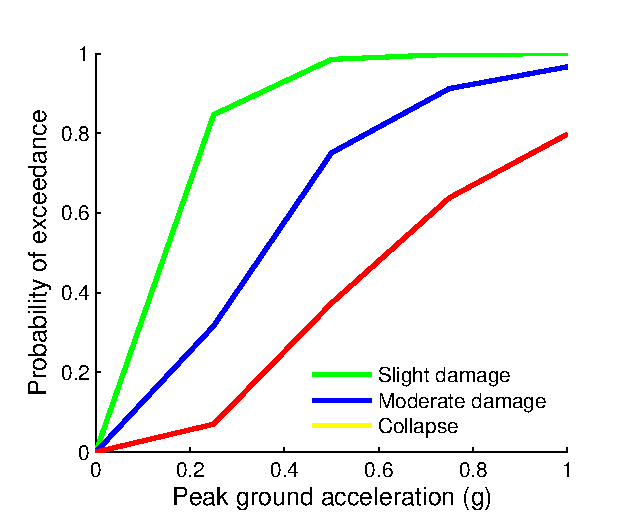
\includegraphics[width=8cm,height=6cm]{./figures/risk/DisFragilityModel.eps}
\caption{Graphical representation of a discrete fragility model.}
\label{fig:fragModelDiscrete}
\end{figure}

Similarly to what was described for the vulnerability models, the NRML schema for this input also has some attributes that are common to all of the fragility functions comprising the model. This initial portion of the schema is depicted below:

\begin{Verbatim}[frame=single, commandchars=\\\{\}, samepage=true]
<?xml version="1.0" encoding="UTF-8"?>
<nrml xmlns:gml="http://www.opengis.net/gml"
      xmlns="http://openquake.org/xmlns/nrml/0.4">
<\textcolor{red}{<fragilityModel format="discrete">}>
    <\textcolor{green}{description} "Fragility Model for RC" <\textcolor{green}{/description}>
    <\textcolor{green}{limitStates} 
        slight damage
        moderate damage
        collapse     
    <\textcolor{green}{/limitStates}>
    ...
\end{Verbatim}

\begin{itemize}
\item  \Verb+description+: represents an attribute that can be used to include  some information about the fragility model, for example, what building typologies are being covered or the source of the fragility model;
\item  \Verb+limitStates+: this field is used to define the number and nomenclature of each limit state. Despite the fact that three limit states are being employed in this example, it is possible to establish any damage scale, as long as a fragility curve is always defined for each limit state. 
\end{itemize}
    
\begin{Verbatim}[frame=single, commandchars=\\\{\}, samepage=true]
    ...  
    <\textcolor{green}{ffs noDamageLimit= 0.05}> 
        <\textcolor{blue}{taxonomy} RC <\textcolor{blue}{/taxonomy}>
        <\textcolor{blue}{IML} IMT="PGA" imlUnit="g"> 0.0 0.25 0.50 0.75 1.00 <\textcolor{blue}{/IML}>
        
        <\textcolor{blue}{ffd} ls="slight damage">
            <\textcolor{magenta}{poes}> 0.0 0.85 0.98 0.99 1.00 < \textcolor{magenta}{/poes}>
        <\textcolor{blue}{/ffd}
        <\textcolor{blue}{ffd} ls="moderate damage">
            <\textcolor{magenta}{poes}> 0.0 0.32 0.75 0.91 0.97 < \textcolor{magenta}{/poes}>
        <\textcolor{blue}{/ffd}
        <\textcolor{blue}{ffd} ls="collapse">
            <\textcolor{magenta}{poes}> 0.0 0.07 0.37 0.64 0.80 < \textcolor{magenta}{/poes}>
        <\textcolor{blue}{/ffd}      
    <\textcolor{green}{/ffs}> 
<\textcolor{red}{/fragilityModel}>  
</nrml>      
\end{Verbatim}

For each building typology, a set of limit state curves need to be stored within the field \Verb+ffs+ (fragility function set). The following attributes are currently being employed to define this input:

\begin{itemize}
\item  \Verb+noDamageLimit+: this attribute defines the intensity measure level below which no damage occurs;  
\item  \Verb+taxonomy+: a unique key that is used to relate each fragility function with the exposure elements; 
\item  \Verb+IML+: this attribute serves the purposes of defining the list of intensity measure levels for which the limit state curves are defined. In addition, it is also necessary to define the intensity measure type (\Verb+IMT+) being used and the respective units (\Verb+imlUnit+);
\item  \Verb+ffd+: this field (fragility function discrete) is used to define the probabilities of exceedance (\Verb+poes+) of each limit state curve. It is also necessary to include which limit state is being defined in the attribute \Verb+ls+.
\end{itemize}

As previously mentioned, user may choose to define the fragility functions in a continuous manner, through the usage of cumulative lognormal functions. In Figure \ref{fig:fragModelContinuous}, a continuous fragility model is presented.

\begin{figure}[ht]
\centering
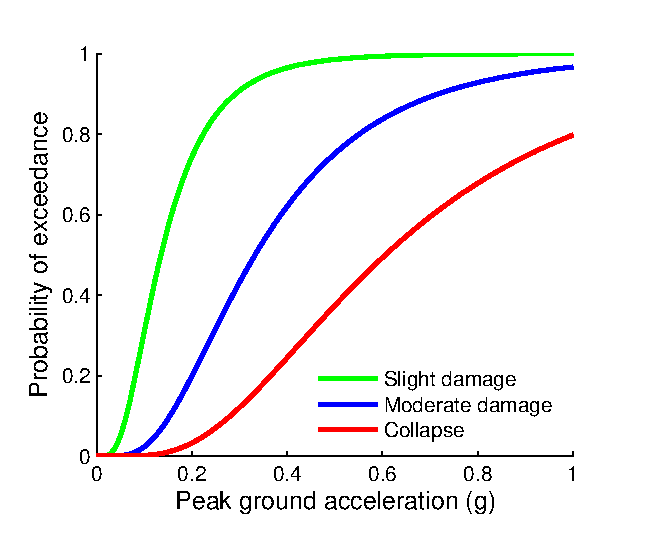
\includegraphics[width=8cm,height=6cm]{./figures/risk/ConFragilityModel.eps}
\caption{Graphical representation of a continuous fragility model.}
\label{fig:fragModelContinuous}
\end{figure}

The NRML schema to store these functions has an initial structure similar to what was described for the discrete fragility models. Then, the continuous limit state curves are stored as illustrated below:

\begin{Verbatim}[frame=single, commandchars=\\\{\}, samepage=true]
    ...  
    <\textcolor{green}{ffs noDamageLimit= 0.05}> 
        <\textcolor{blue}{taxonomy} RC <\textcolor{blue}{/taxonomy}>
        <\textcolor{blue}{IML} IMT="PGA" minIML="0.0" maxIML="1.0" imlUnit="g" ><\textcolor{blue}{/IML}>
        <\textcolor{blue}{ffd} ls="slight damage">
            <params \textcolor{magenta}{mean}="0.16" \textcolor{magenta}{stddev}="0.11" />
        <\textcolor{blue}{/ffd}
        <\textcolor{blue}{ffd} ls="moderate damage">
            <params \textcolor{magenta}{mean}="0.40" \textcolor{magenta}{stddev}="0.26" />
        <\textcolor{blue}{/ffd}
        <\textcolor{blue}{ffd} ls="collapse">
            <params \textcolor{magenta}{mean}="0.73" \textcolor{magenta}{stddev}="0.48" />
        <\textcolor{blue}{/ffd}      
    <\textcolor{green}{/ffs}> 
<\textcolor{red}{/fragilityModel}>
</nrml>        
\end{Verbatim}

Again, the set of limit state curves for each building typology needs to be stored within the field \Verb+ffs+ (fragility function set), through the definition of the following attributes:

\begin{itemize}
\item  \Verb+noDamageLimit+: this attribute defines the intensity measure level below which no damage occurs;
\item  \Verb+type+: this parameter defines the type of probabilistic distribution being used to define the limit state curves. Currently OpenQuake only supports lognormal distributions, however, the capability of considering other types of distributions (e.g. normal, exponential) will be developed in the future;
\item  \Verb+taxonomy+: a unique key that is used to relate each fragility function with the exposure elements; 
\item  \Verb+IML+: in this field, the intensity measure type (\Verb+IMT+) and associated units (\Verb+imlUnit+) for which the limit state curves is defined, along with the minimum (\Verb+minIML+) and maximum (\Verb+maxIML+) intensity measure levels enclosing the range of applicability of the set of fragility functions;
\item  \Verb+ffc+: this field (fragility function continuous) is used to define the mean (\Verb+mean+) and standard deviation (\Verb+stddev+) of the cumulative lognormal function. In addition, the limit state for the curve being defined needs to be specified in the attribute \Verb+ls+.
\end{itemize}

\subsection{Configuration file}
The configuration file represents the location where the paths to the input files, the parameters controlling the risk calculations and the type of outputs are defined. Some initial parameters common to all the risk calculators are presented below. The remaining parameters that are specific to each risk calculator are discussed in subsequent sections. For additional information about how each parameter is being used within the methodologies implemented in the oq-engine, users advised to consult the OpenQuake book. 

\begin{Verbatim}[frame=single, commandchars=\\\{\}, samepage=true]
[general]
description = Scenario Risk Nepal
calculation_mode = scenario

exposure_file = exposure_model.xml
region_constraint = 78.0 31.5,89.5 31.5,89.5 25.5,78 25.5
maximum_distance = 10
...
\end{Verbatim}

\begin{itemize}
\item  \Verb+description+: a parameter that can be used to include some information about the type of calculations that are going to be performed;
\item  \Verb+calculation_mode+: this parameter sets the type of calculations. The key word for each risk calculator is described in the following sections;
\item  \Verb+exposure_file+: this parameter is used to specify the path to the exposure model file;
\item  \Verb+region_constraint+: this field is used to define the polygon enclosing the region of interest. Assets outside of this region will not be considered in the risk calculations. This region is defined using pairs of coordinates (longitude and latitude in decimal degrees) that indicate the vertexes of the polygon;
\item  \Verb+maximum_distance+: this parameter indicates the maximum allowable distance between the asset and the closest hazard input. If no hazard input is found within this distance, the asset is skipped and a message is thrown mentioning the id of the asset affected by this issue.
\end{itemize}

Depending on the type of calculations, other parameters besides the aforementioned ones need to be provided, as it is described in the following sections.

\subsubsection{Scenario Risk Calculator}
In order to run this calculator, the parameter \Verb+calculation_mode+ needs to be set to \Verb+scenario+. The remaining parameters are illustrated bellow.

\begin{Verbatim}[frame=single, commandchars=\\\{\}, samepage=true]
...
vulnerability_file = vulnerability_model.xml
asset_correlation = 0.7
master_seed = 3
\end{Verbatim}

\begin{itemize}
\item  \Verb+vulnerability_file+: this parameter is used to specify the path to the vulnerability model file;
\item  \Verb+asset_correlation+: if the uncertainty in the loss ratios has been defined within the vulnerability model, users can specify a coefficient of correlation that will be used in the Monte Carlo sampling process of the loss ratios, between assets sharing the same taxonomy. If the \Verb+asset_correlation+ is set to one, the loss ratio residuals will be perfectly correlated. On the other hand, if this parameter is set to zero, the loss ratios will be sampled independently. Any value between zero and one will lead to increasing levels of correlation;
\item  \Verb+master_seed+: this parameter is used to control the random generator in the loss ratio sampling process. This way, if the same \Verb+master_seed+ is defined at each calculation run, the same random loss ratios will be generated, thus allowing the replicability of the results.
\end{itemize}

\subsubsection{Scenario Damage Calculator}
For this calculator, the parameter \Verb+calculation_mode+ needs to be defined as \Verb+scenario_damage+. There is only a parameter specific to this calculator, which is the fragility model file path, as presented below.

\begin{Verbatim}[frame=single, commandchars=\\\{\}, samepage=true]
...
fragility_file = fragility_model.xml
\end{Verbatim}

\begin{itemize}
\item  \Verb+fragility_file+: a parameter used to define the path to the fragility model file.
\end{itemize}

\subsubsection{Probabilistic Event-based Risk Calculator}
The parameter \Verb+calculation_mode+ needs to be set to \Verb+event_based+ in order to use this calculator. Similarly to what was described in the Scenario Risk Calculator, a Monte Carlo sampling process is also employed within this module to take into account the loss ratio uncertainty. Hence, the parameters \Verb+asset_correlation+ and \Verb+master_seed+ need to be defined as previously described. The remaining parameters are presented below.

\begin{Verbatim}[frame=single, commandchars=\\\{\}, samepage=true]
...
vulnerability_file = vulnerability_model.xml
asset_correlation = 0.7
master_seed = 3

loss_curve_resolution = 20
conditional_loss_poes = 0.01, 0.05, 0.1
\end{Verbatim}

\begin{itemize}
\item  \Verb+loss_curve_resolution+: since this calculator uses an event-based approach, a large number of levels of loss (and associated probability of exceedance) is computed (one per event) for each asset. Oq-risklib will use this large set of results to extrapolate a loss curve, whose number of points are controlled by the this parameter;
\item  \Verb+conditional_loss_poes+: this parameter is used to define the probabilities of exceedance, used in the calculation of the loss maps.
\end{itemize}

\subsubsection{Classical PSHA-based Risk Calculator}
In order to run this calculator, the parameter \Verb+calculation_mode+ needs to be set to \Verb+classical+. With this calculator it is also possible to extract loss maps, so the parameter \Verb+conditional_loss_poes+ needs to be defined as explained in the previous sub-section. The remaining parameter is illustrated below.
\begin{Verbatim}[frame=single, commandchars=\\\{\}, samepage=true]
...
vulnerability_file = vulnerability_model.xml

lrem_steps_per_interval = 2
conditional_loss_poes = 0.01, 0.05, 0.1
\end{Verbatim}

\begin{itemize}
\item  \Verb+lrem_steps_per_interval+: this parameter controls the number of intermediate values between consecutive loss ratios (as defined in the vulnerability model) that are considered in the risk calculations. A larger number of loss ratios than the ones defined in each vulnerability function are considered, in order to better account for the uncertainty in the loss ratio distribution.  
\end{itemize}

\subsubsection{Benefit/Cost Ratio Calculator}
As previously explained, this calculator uses loss exceedance curves which can be calculated using the Classical PSHA-based Risk or the Probabilistic Event-based Risk calculators. Therefore, depending on which calculator a user chooses to employ, the configuration file will be different. If the Classical PSHA-based Risk calculator is employed, then the \Verb+calculation_mode+ should be set to \Verb+classical_bcr+ and the calculator-specific part of the configuration file should be defined as presented below.

\begin{Verbatim}[frame=single, commandchars=\\\{\}, samepage=true]
...
vulnerability_file = vulnerability_model.xml
vulnerability_retrofitted_file = vulnerability_model_retrof.xml

lrem_steps_per_interval = 2

interest_rate= 0.005
asset_life_expectancy = 50
\end{Verbatim}

\begin{itemize}
\item  \Verb+vulnerability_retrofitted_file+: this parameter is used to specify the path to the vulnerability model file containing the vulnerability functions for the retrofitted version of the assets;  
\item  \Verb+interest_rate+: this parameter represents the interest rate and it serves the purposes of taking into account the variation of building value throughout the time;
\item  \Verb+asset_life_expectancy+: this variable defines the life expectancy of the assets.
\end{itemize}

Alternatively, if a user decides to employ the Probabilistic Event-based Risk calculator for the calculation of the loss curves, then the \Verb+calculation_mode+ should be set to \Verb+event_based_bcr+ and the remaining portion of the configuration file should be defined as follows.

\begin{Verbatim}[frame=single, commandchars=\\\{\}, samepage=true]
...
vulnerability_file = vulnerability_model.xml
vulnerability_retrofitted_file = vulnerability_model_retrof.xml
asset_correlation = 0.7
master_seed = 3

loss_curve_resolution = 20

interest_rate= 0.005
asset_life_expectancy = 50
\end{Verbatim}